\section{Approach}
\label{sec:approach}
In this section, we first describe our methodology for 
cause-effect pairs extraction. 
Then we demonstrate the global causal attention as well as its fusion mechanism based on the CNN seq2seq model for commonsense causality generation.

\subsection{Cause-Effect Pairs Extraction}
The sentences are the basic semantic units which completely describe the events with both \emph{agents} and \emph{actions}.
Therefore, to study the causal sentence generation task, we build a new dataset of cause-effect sentence pairs from novels~\footnote{We describe this corpus in detail in \secref{sec:eval}.} by extracting main and subordinate clauses connected by causal conjunctions (i.e., ``because'' and ``so''). 
We perform the extraction as follows:

\begin{figure}[t!]
	\centering
	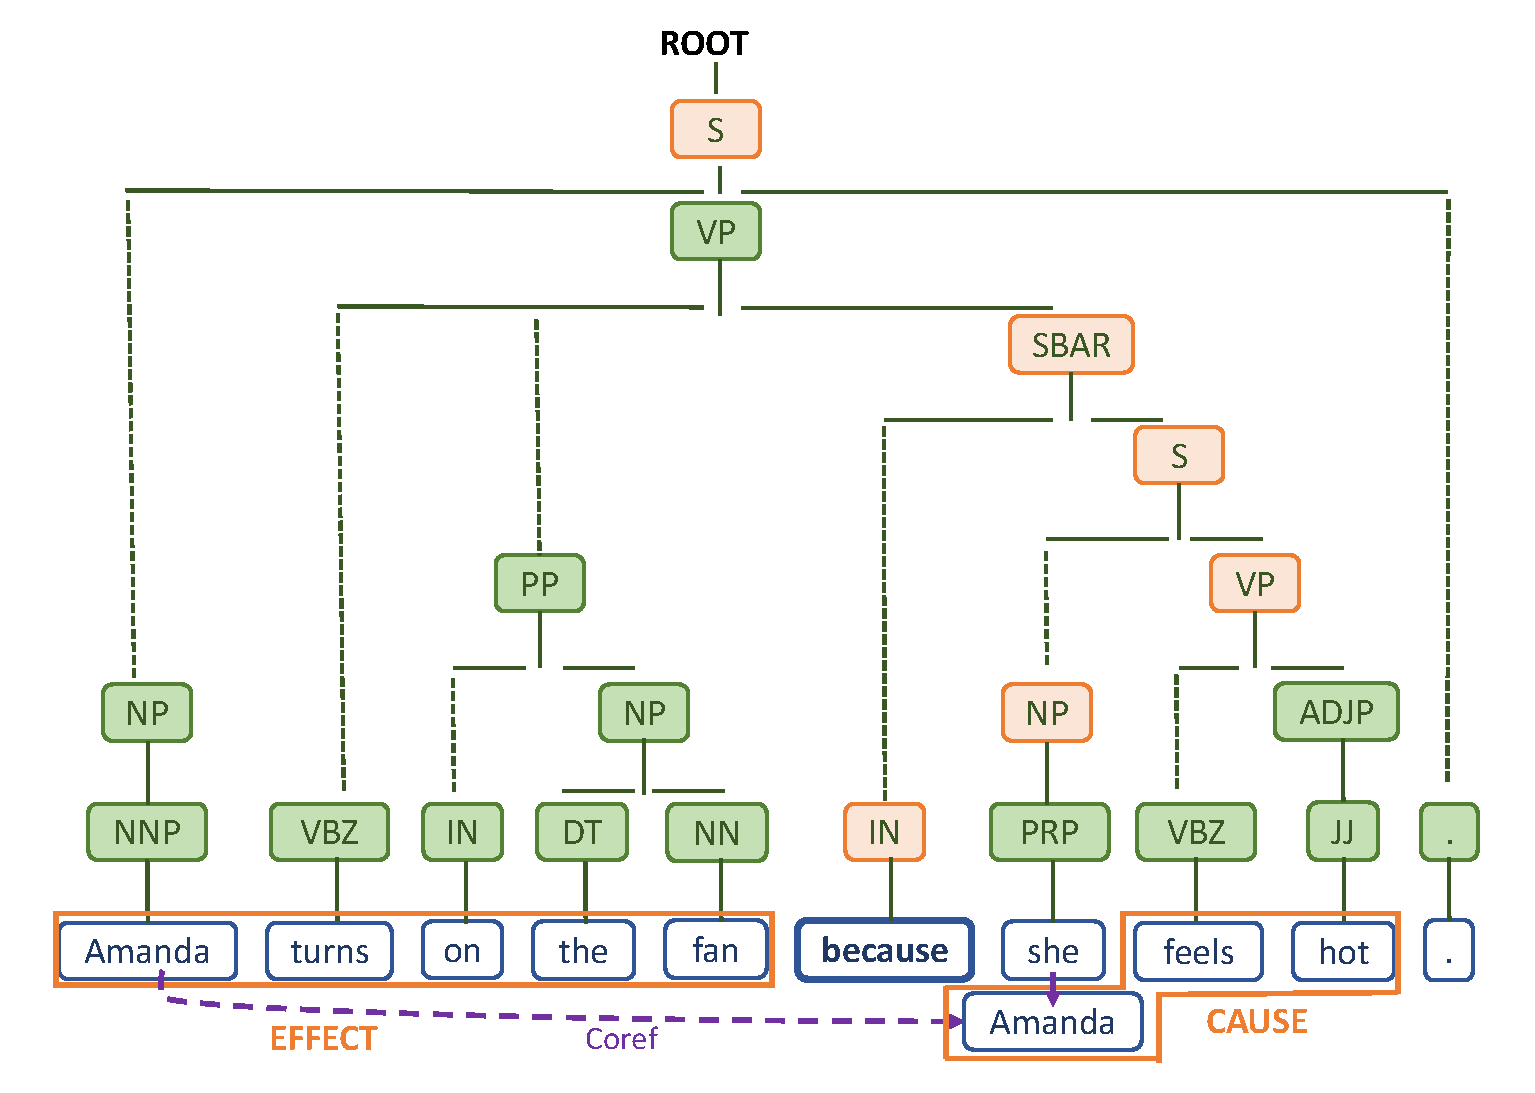
\includegraphics[width=\columnwidth]{parse.pdf}
	\caption{Cause and effect sentence extracted from a sample sentence after coreference resolution, along with its constituent parse tree. Nodes coloured in light orange are those critical for syntactical checking in our extraction process.}
	\label{fig:parse}
\end{figure}
\begin{itemize}
	\item Cue Sentences Collection. 
	We first collect sentences containing ``because'' or ``so'' by regular expression matching. Those sentences are fed into Stanford CoreNLP~\cite{stanfordcorenlp} tools for tokenization, POS tagging, constituent parsing and dependency parsing.
	\item Negation Detection. 
	If the causal conjunction node in dependency tree
	has a negation word sibling such as ``not'' and ``n't'', 
	we do not consider this sentence for further extraction.
	\item Clause Detection. 
	We design syntactic pattern matching rules for 
	cause-effect sentence pairs extraction.
	 Basically we make sure the "because" in the sentence is a subordinate conjunction word leading a subordinate clause(tagged as `SBAR'), which contains a declarative 
	sentence(`S') with subject(`NP') and predicate(`VP').
	Similarly, we design the syntactic rules for the `so that' pattern.
	We further demonstrate such syntactic rules in \figref{fig:parse}.
	
	\item Spans Extraction. 
	We remove redundant punctuations and unwanted sentence
	constituents from the subtree of the main clause and that of the subordinate clause. Then, the text spans contained by those subtrees are extracted as cause-effect sentence pairs.
%	\item (Partial) Coreference Resolution. The order of cause/effect span is determined by the causal conjunction. Take ``because'' as an example, the order is always ``EFFECT because CAUSE'', resulting in representative mention in effect sentence but 
%	pronouns in cause. Therefore, we substitute pronouns in subordinate clause with the representative mention in main clause for each causal pair to enable bidirectional 
%	inference. We don't do coreference resolution on the whole sentence to avoid unnecessary repetition. 

\end{itemize}

\textbf{Input Transformations.} 
We create two data examples from each cause-effect sentence pair for both forward causal reasoning and backward causal reasoning.
While training, we add the special token $\left< f\right>$ or $\left< b \right>$ in front of the target span to indicate the forward or backward reasoning example.
When testing, we initialize the first token of the generated sequence as $\left< f\right>$ or $\left< b \right>$  to perform the forward reasoning or backward reasoning separately.

Note that, we also do the co-reference resolution for the cue sentences, since we create both forward and backward reasoning examples. 
Finally, we create two source/target pairs from the example sentence shown in \figref{fig:parse} as follows:

\textbf{Forward:}
 \begin{itemize}
	\item [] source sequence: Amanda feels hot
	\item [] target sequence: $\left< f\right>$ Amanda turns on the fan
\end{itemize}

\textbf{Backward:}
\begin{itemize}
	\item [] source sequence: Amanda turns on the fan
	\item [] target sequence: $\left< b\right>$ Amanda feels hot
\end{itemize}
%\YZ{co-reference}

\subsection{Background: CNN Seq2seq Model}
\label{sec:cnn}
In this section, we briefly introduce the convolutional sequence to sequence (CNN seq2seq\footnote{\url{https://github.com/facebookresearch/fairseq-py}}) model and later we implement our proposed attention mechanism on this model.

%\begin{figure}[th]
%	\centering
%	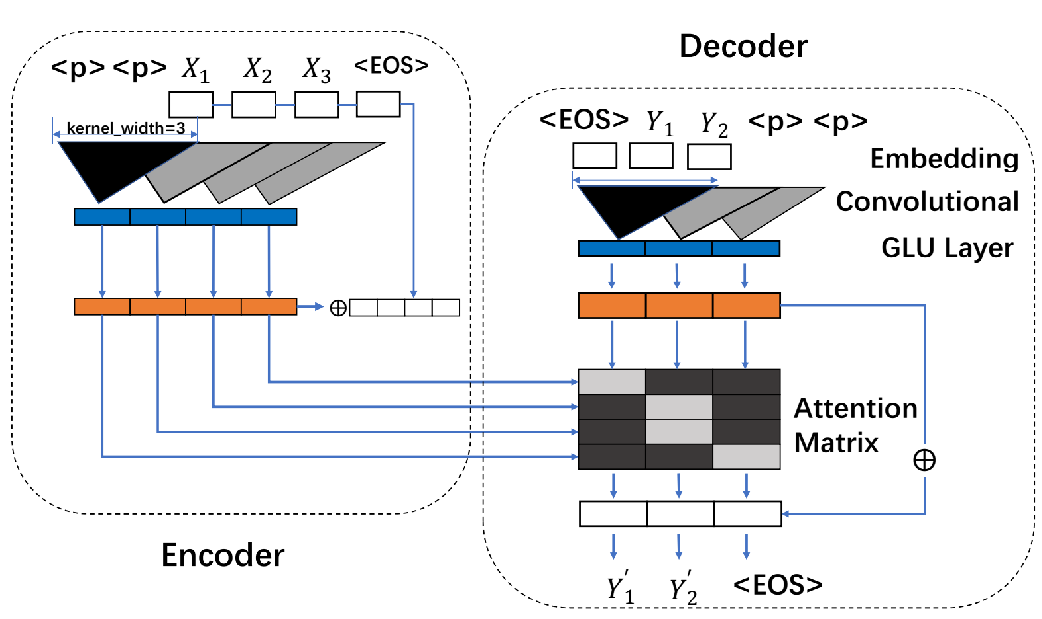
\includegraphics[width=1.0\columnwidth]{cnn}
%	\caption{Convolutional seq2seq model. }
%	\label{fig:basicModel}
%\end{figure}
%
%The CNN seq2seq model includes multi-layer convolutional seq2seq networks \cite{gehring2017convs2s} and attention mechanism \footnote{\url{https://github.com/facebookresearch/fairseq-py}}
%(\figref{fig:basicModel}).

In CNN seq2seq models, given the input elements $\textbf{x} = (x_{1},x_{2},...,x_{m})$ and 
output elements $\textbf{y} = (y_{1}, y_{2},..., y_{n})$ ($m>n$),
we obtain the input representations  $\mathbf{X} = (X_1,...,X_m)$ 
and output representations $\mathbf{Y}=(Y_1,...,Y_n)$ by combining
word embeddings and their corresponding position embeddings vectors. 
$\mathbf { z } ^ { l } = \left( z _ { 1 } ^ { l } , \ldots , z _ { m } ^ { l } \right)$ and $\mathbf { h } ^ { l } = \left( h _ { 1 } ^ { l } , \ldots , h _ { n } ^ { l } \right)$ 
are convolutional output of the encoder and decoder in the $l$-th layer.
We use GLU \cite{DauphinFAG17} and residual connections \cite{HeZRS16} after convolution 
in each layer to ensure that the sufficient and effective information is transmitted layer by layer.  
\begin{equation}
%\small
h _ { i } ^ { l } = ~ GLU \left( W ^ { l } \left[ h _ {i-k/2 } ^ { l - 1 } , \ldots , h _ { i+k/2 } ^ { l - 1 } \right] + b _ { w } ^ { l } \right)  + h _ { i } ^ { l - 1 }
\end{equation} 
where \textit{k} is kernel width.
We compute the probability
distribution of generating the next elements $y_{i+1}$
based on the current state and transform the top
decoder output $h_{i}^{l}$ via softmax:
%\begin{equation}
%%\small
%\begin{split}
%p \left( y _ { i + 1 } | y _ { 1 } , \ldots , y _ { i } , \mathbf { x } \right) = 
%& \operatorname { softmax } \left( W _ { o } h _ { i } ^ { L } + b _ { o } \right) \\ 
%&\in \mathbb { R } ^ { T }
%\end{split}
%\end{equation}
\begin{equation}
%\small
p \left( y _ { i + 1 } | y _ { 1 } , \ldots , y _ { i } , \mathbf { x } \right) = 
 \operatorname { softmax } \left( W _ { o } h _ { i } ^ { L } + b _ { o } \right) \\ 
\in \mathbb { R } ^ { T }
\end{equation}
For each decoder layer, 
we combine the current decoder state $h_{i}$
with an embedding of the previous target element via $Y_{i}$:
\begin{equation}
%\small
d _ { i } ^ { l } = W _ { d } ^ { l } h _ { i } ^ { l } + b _ { d } ^ { l } + Y _ { i }
\end{equation}

The conditional input to the current 
decoder layer is a weighted sum of both encoder states and input element representations.
\begin{equation}\label{eq:a}
%\small
a _ { i j } ^ { l } = \frac { \exp \left( d _ { i } ^ { l } \cdot z _ { j } ^ { u } \right) } { \sum _ { t = 1 } ^ { m } \exp \left( d _ { i } ^ { l } \cdot z _ { t } ^ { u } \right) }
\end{equation}
\begin{equation}\label{eq:c}
%\small
c _ { i } ^ { l } = \sum _ { j = 1 } ^ { m } a _ { i j } ^ { l } \left( z _ { j } ^ { u } + X_j \right)
\end{equation}
%where $z_{j}^{u}$ is the encoder output of last layer $u$.  
where $u$ is the last layer of encoder.  
Finally, $c _ { i } ^ { l }$ is added to $h_{i}^{l}$ as the input for the next decoder layer.


\subsection{Global Causal Attention}
In this section, we propose the global causal attention mechanism as the guidance for causality generation.

Specifically, we use the word-level causal strengths (i.e. $cs$)~\cite{} in logarithm space as the attention scores which carries the causal dependency in global manner.
The logarithm causal strength (i.e. $CS$) is computed as:
%\begin{equation}\label{eq:acs}
%	\begin{split}
%	CS(y_i, x_j)  & =  \log\left(cs(y_i,x_j)\right) \\
%		& - \log\left(min\{cs(\cdot, \cdot)\}\right)
%	\end{split}
%\end{equation}
\begin{equation}\label{eq:acs}
CS(y_i, x_j) = \log\left(cs(y_i,x_j)\right) - \log\left(min\{cs(\cdot, \cdot)\}\right)
\end{equation}

\begin{equation}
\label{eq:causal_attn}
a _ { i j }= Softmax\left( CS(y_i, x_j) \right) ,
\end{equation}
where $y_i$ is $i$-th word in encoder input, 
and $x_j$ is $j$-th word in decoder output.

For the vanilla global causal attention, 
we simply replace the attention scores in \eqnref{eq:a} with \eqnref{eq:causal_attn}.

%\subsection{Causality Fused Attention Mechanism}
\subsection{Causal Attention Fusion Mechanism}
\label{sec:fusion}
In the previous section, the global causal attention scores do not change across different layers which loses the hierarchical semantic attending information.
Thus, we propose a novel attention fusion mechanism 
to integrate the global causal attention with the stacked soft attention. In this section, we describe two attention fusion mechanisms used for our experiments.

To facilitate causality generation, 
we propose two attention fusion mechanisms as follows,
equipping the CNN seq2seq model with global causal information.
%To facilitate causality generation, we propose \emph{causal weighing} $P_{cs}$ to fuse the global causal attention 
%with soft attention, changing \eqnref{eq:a} and \eqnref{eq:c} as follows:

\textbf{Easy Attention Fusion.}
To weigh global causal attention score and soft attention score, we uses the \emph{causal fusion weight} $p_{cs}$  as follows:
\begin{equation}
\label{eq:easy}
a_{ij} = p_{cs} \cdot CS(y_i,x_j) + (1-p_{cs}) \cdot a_{ij}
\end{equation}
We compute the fusion attention scores as shown in \eqnref{eq:easy}, weighing the global causal attention and soft attention equally by setting $p_{cs}$ as a fixed value $0.5$. 

\textbf{Causal Weighing Attention Fusion.} 
In the \emph{easy attention fusion} mechanism, the combination of attention scores are fixed across different encoder and decoder states.

Our causal weighing attention fusion mechanism is designed to aggregate causal information from the global and local causal dependency to refine the decoding at every time step. 
We redesign $p_{cs}$ as the learnable weights for decoding time steps. 
The causal weight at the $i$-th decoding time step ($p^{(i)}_{cs}$) is calculated based on the encoder context state ($\mathbf{c_i}$) and decoder state ($\mathbf{b_i}$) as follows:
\begin{equation}
p^{(i)}_{cs} = \sigma(\mathbf{W}^e\mathbf{c_i} + \mathbf{W}^d\mathbf{d_i}) 
\end{equation}

\begin{equation}
\mathbf{e_i} = \sum_{j=1}^{m}a_{ij}\mathbf{z_j},
\end{equation}
where $\mathbf{e_i}$ is the context vector when decoding at the $i$-th time step. 
$p^{(i)}_{cs}$ weighs the contribution of the global causal attention and the local soft attention at the $i$-th decoding time step according to the dependency between the current decoder hidden state and all the encoder hidden states.
We use the global causal attention to summary the
encoder hidden states, the weights the contribution 

%\begin{equation}
%\begin{split}
%c_i = & ~P^{(i)}_{cs}W_{cs}\sum_{j=1}^{m}CS(y_i,x_j)z_{ij} \\
%		& + (1-P^{(i)}_{cs})e_i 
%\end{split}
%\end{equation}

\begin{equation}
%\begin{split}
\mathbf{c_i} = p^{(i)}_{cs}\mathbf{w_{cs}}\sum_{j=1}^{m}\mathbf{v_{\boldsymbol{\cdot} j}} \times \mathbf{z_j}  + (1-p^{(i)}_{cs})\mathbf{e_i},
%\end{split}
\end{equation}
where $v_{\cdot j}$ is the causal strength vector with $V \times 1$ dimension  $\mathbf{w_{cs}}$ is 
\begin{figure*}[th]
    \centering
    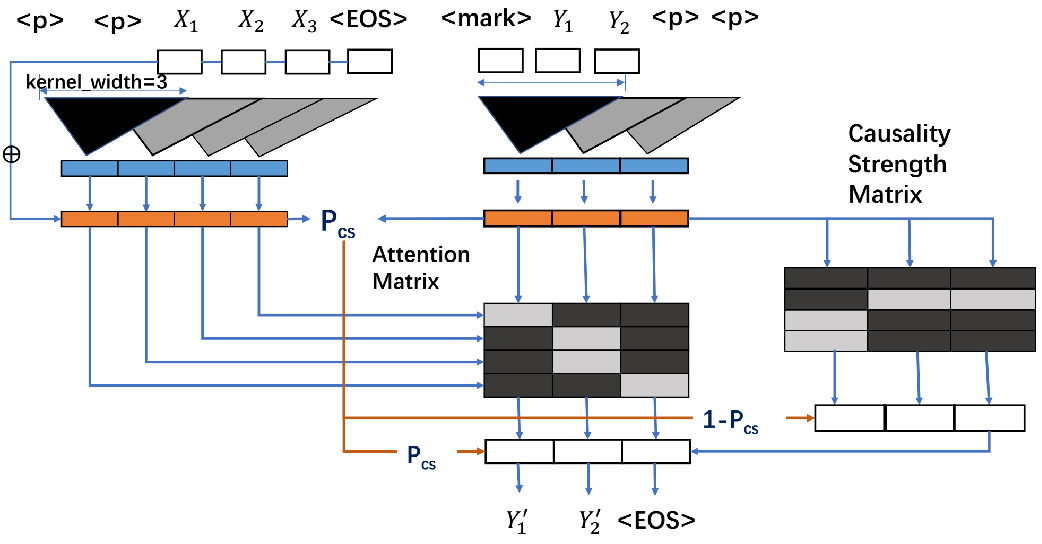
\includegraphics[width=1.5\columnwidth]{fusedatt}
    \caption{Causality Fused attention. }
    \label{fig:fusedatt}
\end{figure*}
The causality fused attention mechanism is illustrated in \figref{fig:fusedatt}.
Compared with Global and Easy Combination methods, the advatages
of Fusion attention is that this model has the ability to 
obtain the causality information and generate correct text according
to desired \textit{marks} in its inner state.



To enable the user to generate desired text (cause or effect), 
we first set two \textit{marks} $<b>$ and $f$, 
repectively representing the generation of cause and effect. 
We then expand the input vocabulary with these two \textit{marks} 
indicate the desired type. For training,
we prepend the input of our summarizer with a \textit{mark} 
that indicates the causality relation between input and output.
At test time, we control type of generated
text by prepending a particular \textit{marker} token.
To provide causality information to CNN seq2seq model,
we propose three methods as follows:
